% !Mode:: "TeX:UTF-8"
\documentclass{article}
% !Mode:: "TeX:UTF-8"
\usepackage[english]{babel}
\usepackage[UTF8]{ctex}
\usepackage{amsmath, amsthm, amssymb}

% Figure
\usepackage{graphicx}
\usepackage{float} %% H can fix the location
\usepackage{caption}
\usepackage[format=hang,singlelinecheck=0,font={sf,small},labelfont=bf]{subfig}
\usepackage[noabbrev]{cleveref}
\captionsetup[subfigure]{subrefformat=simple,labelformat=simple,listofformat=subsimple}
\renewcommand\thesubfigure{(\alph{subfigure})}

\usepackage{epstopdf} %% convert eps to pdf
\DeclareGraphicsExtensions{.eps,.mps,.pdf,.jpg,.png} %% bmp, gif not supported
\DeclareGraphicsRule{*}{eps}{*}{}
\graphicspath{{img/}{figure/}{../figure/}} %% fig directorys

%% \usepackage{pstricks} %% a set of macros that allow the inclusion of PostScript drawings directly inside TeX or LaTeX code
%% \usepackage{wrapfig} %% Wrapping text around figures

% Table
\usepackage{booktabs} %% allow the use of \toprule, \midrule, and \bottomrule
\usepackage{tabularx}
\usepackage{multirow}
\usepackage{colortbl}
\usepackage{longtable}
\usepackage{supertabular}

\usepackage[colorinlistoftodos]{todonotes}

% Geometry
\usepackage[paper=a4paper, top=1.5cm, bottom=1.5cm, left=1cm, right=1cm]{geometry}
%% \usepackage[paper=a4paper, top=2.54cm, bottom=2.54cm, left=3.18cm, right=3.18cm]{geometry} %% ms word
%% \usepackage[top=0.1cm, bottom=0.1cm, left=0.1cm, right=0.1cm, paperwidth=9cm, paperheight=11.7cm]{geometry} %% kindle

% Code
%% \usepackage{alltt} %% \textbf can be used in alltt, but not in verbatim

\usepackage{listings}
\lstset{
    backgroundcolor=\color{white},
    columns=flexible,
    breakatwhitespace=false,
    breaklines=true,
    captionpos=tt,
    frame=single, %% Frame: show a box around, possible values are: none|leftline|topline|bottomline|lines|single|shadowbox
    numbers=left, %% possible values are: left, right, none
    numbersep=5pt,
    showspaces=false,
    showstringspaces=false,
    showtabs=false,
    stepnumber=1, %% interval of lines to display the line number
    rulecolor=\color{black},
    tabsize=2,
    texcl=true,
    title=\lstname,
    escapeinside={\%*}{*)},
    extendedchars=false,
    mathescape=true,
    xleftmargin=3em,
    xrightmargin=3em,
    numberstyle=\color{gray},
    keywordstyle=\color{blue},
    commentstyle=\color{green},
    stringstyle=\color{red},
}

% Reference
%% \bibliographystyle{plain} % reference style

% Color
\usepackage[colorlinks, linkcolor=blue, anchorcolor=red, citecolor=green, CJKbookmarks=true]{hyperref}
\usepackage{color}
\def\red#1{\textcolor[rgb]{1.00,0.00,0.00}{#1}}
\newcommand\warning[1]{\red{#1}}

% Other
%% \usepackage{fixltx2e} %% for use of \textsubscript
%% \usepackage{dirtree}  %% directory structure, like the result of command tree in bash shell

   %导入需要用到的package
% !Mode:: "TeX:UTF-8"
%+++++++++++++++++++++++++++++++++++article+++++++++++++++++++++++++++++++++
%customize the numbering of equation, to make it like section-subsection-equation style, for example,1-2-3
\makeatletter\@addtoreset{equation}{subsection}\makeatother
\renewcommand\theequation{%
\thepart\arabic{section}%
-\thepart\arabic{subsection}%
-\thepart\arabic{equation}%
}
%theorem
\newtheorem{definition}{D\'efintion} %% 整篇文章的全局编号
\newtheorem*{thmwn}{Thm} %% without numbers
\newtheorem{theorem}{Th\'eor\`eme}[section] %% 从属于section编号
\newtheorem{corollary}{Corollary}[theorem] %% 从属于theorem编号
\newtheorem{lemma}{Lemma}
\newtheorem{proposition}{Proposition}[section]
\newtheorem{example}{Example}
\newtheorem*{attention}{Attention}
\newtheorem*{note}{Note}
\newtheorem*{remark}{Remark}
\newtheorem{question}{Question}[section]
\newtheorem{problem}{Problem}
\newtheorem{fact}{Fact}

   %导入需要用到的package
\begin{document}
\title{Data Mining \\ Concepts and Techniques \\Eric's Notes}
\author{Eric}
\maketitle
\newpage
\tableofcontents
\newpage
\section{引论}
数据挖掘是一个多学科的交叉领域.\\
统计学, 机器学习, 神经网络, 模式识别, 知识库系统, 信息检索, 高性能计算和可视化等学科

丰富的数据类型:
流, 序列, 图, 时间序列, 符号序列, 生物学序列, 空间, 音频, 图像和视频数据

高级数据库系统: 扩充关系的, 面向对象的, 对象-关系的和演绎的模型. 包括空间的, 时间的, 多媒体的, 主动的, 流和传感器的, 科学和工程数据库, 知识库, 办公信息库在内的面向应用的数据库系统百花齐放

\textbf{数据仓库}\\
一种多个异构数据源在单个站点以统一的模式组织的存储, 以支持管理决策.\\
数据仓库技术包含数据清理, 数据集成和联机分析处理OLAP\\
OLAP是以各种分析技术, 具有汇总, 合并和具体记忆从不同的角度观察信息的能力. 尽管OLAP 工具支持多维分析和决策, 但是对于深层次的分析, 仍然需要其他分析工具, 如提供数据分类, 聚类, 离群点/异常检测和刻画数据随时间变化等特征.

OLAP 操作的列子包括下钻(drill-down) 和上卷(roll-up), 允许用户在不同的汇总级别观察数据\\
例如, 可以对按季度汇总的数据下钻, 观察按月汇总的数据. 类似的, 可以对按城市汇总的数据上卷, 观察按国家汇总的数据

\textbf{可挖掘什么类型的模式}\\
特征化与区分, 频繁模式(频繁项集, 频繁子序列, 频繁子结构), 关联和相关性挖掘, 分类和回归, 聚类分析, 离群点分析.\\
数据挖掘功能用于指定数据挖掘任务发现的模式, 一般而言, 这些任务分为: 描述性(descriptive)和预测性(predictive)

\textbf{关联规则}\\
关联规则从一个侧面揭示了事务之间的某种联系.\\
支持度和置信度总是伴随着关联规则存在的,它们是对关联规则的必要的补充\\
对某条关联规则而言,如 $A \rightarrow B (support=30\%, confidence= 60\%)$\\
其中的$support=30\%$是说, 在所有的事务中同时出现A和B的概率.\\
而$confidence=60\%$是说,所有事务中,在出现A的情况下出现B的概率,即条件概率.
$$
Support(X=>Y) = P(X \eqnote{and} Y) \eqspace
Confidence(X=>Y) = P(Y | X)
$$
$$Buys(X, "computer") \Rightarrow buys (X,"software") [support = 1\%, confidence = 50\%]$$
这个关联规则涉及单个重复的属性或谓词(buys), 单维关联规则 single-dimensional association rule

置信度揭示了A出现时,B是否一定会出现,如果出现则其大概有多大的可能出现.如果置信度为$100\%$,\\
则说明了A出现时,B一定出现.那么,对这种情况而言,假设A和B是市场上的两种商品,就没有理由不进行捆绑销售了.

用于预测分析的分类和回归\\
导出的模型可以用多种形式表示, 如分类规则(即if-then 规则), 决策树, 数学公式或神经网络\par
离群点分析或异常挖掘\\
数据集中可能包含一些数据对象, 他们与数据的一般行为或模型不一致. 这些数据对象是离群点(outlier).\\
大部分的数据挖掘方法都将离群点视为噪声或异常而丢弃, 然而, 在一些应用中(例如, 欺诈检测), 罕见的事件可能比正常出现的事件更令人感兴趣.

\textbf{机器学习}
\begin{itemize}
\item 监督学习Supervised learning: 基本上是分类的同义词
\item 无监督学习 unsupervised learning: 基本上是聚类的同义词
\item 半监督学习 semi-supervised learning, 标记的实例用来学习类模型, 而未标记的实例用来进一步改进类边界
\item 主动学习
\end{itemize}

数据挖掘算法的有效性和可伸缩性\par
增量数据挖掘

\section{认识数据}
\subsection{属性类型}
\textbf{标称属性}nominal attribute: 值是一些符号或事物的名称. 每个值代表某种类别, 编码或状态. 又被称为分类的(categorical) 或枚举的(enumeration)
\textbf{二元属性}binary attribute: 一种标称属性, 两个状态, 通常用0和1 或false, true表示\\
对称二元属性: 两种状态具有同等价值并且携带相同的权重\\
非对称二元属性:
\textbf{序数属性}ordinal attribute: 其可能的值之间具有有意义的序或秩排序ranking, 但是相继值之间的差是未知的\\
例如, 成绩可以用A+, A, A-, B+ 等划分, 意味着排序, 但是划分值之间的差别未明确
\textbf{数值属性}numeric attribute: 可度量的量\\
	区间标度属性interval-scaled: 用相等的单位尺度度量, 可以比较差, 但是没有真正的零点, 例如日期, 我们可以说两个日期相差多少时间, 但是对于0日期, 没有具体的含义\\
	比率标度属性ratio-scaled: 具有固定零点的数值属性, 也就是说, 我们可以说一个值是另一个值的倍数(或比率). 此外, 这些值是有序的, 因此可以计算值之间的差, 均值, 中位数和众数\\
	开氏温标具有绝对零点\par
标称, 二元和序数属性都是定性的

\textbf{离散属性和连续属性}(在文献中, 术语数值属性与连续属性通常可以互换地使用)

\subsection{基本统计描述}
\textbf{中心趋势度量}: 均值(平均值), 加权平均, 截尾均值, 中列数midrange(最大与最小值的平均值), 中位数(中间值), 众数(最常见的值)\\
	正倾斜:\\
	负倾斜
\textbf{数据的散布}: 极差, 四分位数, 四分位数极差, 无数概括和盒图, 方差和标准差

有助于在数据预处理时填补缺失值, 光滑噪声, 识别离群点.\\
数据可视化: 散点图矩阵, 树图\\
数据对象的相似性和相异性\\
最近邻分类, 邻近性度量

极差: $max – min$ \\
\textbf{分位数}quantile: 取自数据分布的每隔一定间隔上的点, 把数据划分成数量上大小基本相等的连贯集合\\
给定数据分布的第$k$ 个q-分位数是值$x$, 使得小于$x$ 的数据值最多为$k/q$, 而大于x的数据值最多为$(q-k)/q$, 其中$k$为整数, 使得$0<k<q$. 我们有$q-1$ 个q-分位数.
2-分位数是一个数据点, 把数据分布划分为高低两半, 对应于中位数\\
4-分位数是3个数据点, 他们把数据分布划分为4 个相等的部分, 使得每部分表示数据分布的四分之一. 通常把他们成为4分位数quartile\\
第一个四分位数记作$Q_1$, 第三个四分位数记为$Q_3$, 四分位数极差$IQR = Q_3 – Q_1$\\
100-分位数通常称为百分位数(percentile)

\textbf{五数概括, 盒图和离群点}\\
识别可疑的离群点的通常规则: 挑选落在第3 个四分位数之上或第1 个四分位数之下至少$1.5 * IQR$ 处的值\par
五数概括(five-number summary)由中位数$Q_2$, 四分位数$Q_1$, $Q_3$, 最小和最大值, 按次序
$Minimum, Q_1, median, Q_3, maximum$\par
盒图(如图\ref{fig.hetu}): 盒的端点在四分位数上, 盒的长度为IQR; 中位数标在盒内; 盒外的两条线(胡须) 延伸到最小和最大值\\
\begin{figure}[htbp]
  \centering
  % Requires \usepackage{graphicx}
  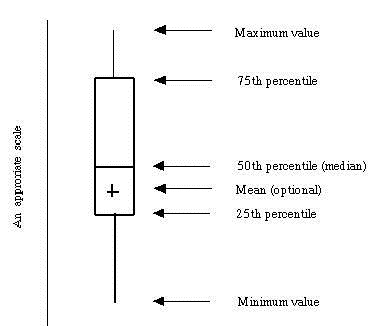
\includegraphics[scale=0.5]{hetu}\\
  \caption{盒图}
  \label{fig.hetu}
\end{figure}

盒图可在$O(nlgn)$时间内计算, 依赖于所要求的质量, 近似盒图可在线性或者子线性时间内计算.

分位数图quantile plot
直方图histogram或频率直方图frequency histogram\\
散点图scatter plot: 确定两个数值变量是否存在联系, 模式或趋势的最有效的图形方法之一\\

\subsection{数据可视化}
\begin{itemize}
\item 基于像素的可视化技术pixel-oriented technique
几何投影可视化技术
	\begin{itemize}
	\item 散点图
	\item 散点图矩阵
    \item 平行坐标parallel coordinates
	\end{itemize}
\item 基于图符icon-based的可视化技术
	\begin{itemize}
	\item 切尔诺夫脸chernoff faces
	\item 人物线条画
	\end{itemize}
\item 层次可视化技术
	\begin{itemize}
	\item 世界中的世界
	\item 树图tree-map
	\end{itemize}
\item 可视化复杂对象和关系
	\begin{itemize}
	\item 标签云tag cloud
	\end{itemize}
\end{itemize}
	
\subsection{度量数据的相似性与相异性}
相似性和相异性都成为紧邻性proximity\\
数据矩阵和相异性矩阵\\
$n$ 个对象, $p$ 个属性\\
数据矩阵data matrix $n \times p$\\
$$
\eqnote{data matrix}_{ij} = x_{ij}
$$
$x_{ij}$ 第$i$ 个对象的第$j$ 个属性的值

相异性矩阵 dissimilarity matrix; $n \times n$
$$
sim(i,j) = 1 – d(i,j)
$$
数据矩阵由两种实体(行的对象,列的属性)组成, 因而被称为二模(two-mode)矩阵\\
相异性矩阵只包含一种实体, 因而被称为单模(one-mode)矩阵\\

许多聚类和最近邻算法都在相异性矩阵上运行

\textbf{标称属性的邻近性度量}
$$
d(i,j) = \frac{p – m}{p}
$$
$m$: 匹配的数目(即对象i和j 取相同状态的属性数)\\
$p$: 属性总数

\textbf{数值属性的相异性}\par
\begin{itemize}
\item 欧几里得距离
\item 曼哈顿距离, 街区距离, 两个点在标准坐标系上的绝对轴距总和
\item 闵可夫斯基距离, $L_p$ 范数
\item 上确界距离(又称为$L_{\infty}$ 范数和切比雪夫Chebyshev距离)
\end{itemize}

\textbf{序数属性}:转化为数值属性进行度量

混合类型属性的相异性

\subsubsection{余弦相似性}
词频向量term frequency vector 通常很长, 并且是稀疏的\\
使用这种结构的应用包括信息检索, 文本文档聚类, 生物学分类和基因特征映射.\\
对于这类稀疏的数值数据, 前面介绍过的传统的距离度量效果并不好

余弦相似性是一种度量, 他可以用来比较文档, 或针对给定的查询词向量对文档排序
$$sim(x,y) = \dfrac{x \cdot y}{\norm{x} \norm{y}}$$

当属性为二元属性时, 余弦相似性衡量的是他们共享的属性

\section{数据预处理}
数据质量: 准确性, 完整性, 一致性, 时效性, 可信性和可解释性.

\subsection{数据清理data cleaning}
用来清除数据中的噪声, 填补缺失的值, 识别或删除离群点并解决不一致性.

填充缺失值的方法:忽略元组, 人工填写缺失值,使用一个全局常量填充缺失值, 使用属性的中心度量(如均值或中位数)填充缺失值, 使用与给定元组属同一类的所有样本的属性均值或中位数,使用最可能的缺失值填充缺失值(用回归,贝叶斯形式化方法的基于推理工具或决策树归纳确定)

噪声noise: 是被测量的变量的随机误差或方差.

数据光滑技术
\begin{description}
	\item [分箱binning] 通过考察数据的近邻(即周围的值)来光滑有序数据值,将数据划分到等频的箱中, 局部光滑方法, 有用箱均值光滑(用箱中数据的均值代替箱中的每一个值), 用箱中位数光滑, 用箱边界光滑
	\item [回归regression] 用一个函数拟合数据来光滑数据
	\item [离群点分析outlier analysis] 可以通过聚类来检测离群点
\end{description}

唯一性规则, 连续性规则和控制规则

数据清洗工具data srubbing tool, 数据审计工具data auditing tool, 数据迁移工具data migration tool. ETL(extraction/transformation/loading), Potter's Wheel 一个公开的数据清理工具, 集成了偏差检测和数据变换

\subsection{数据集成data integration}
将数据由多个数据源合并成一个一致的数据存储, 如数据仓库.
\subsubsection{冗余和相关分析}
一个属性如果能够由另外一个属性导出, 则这个属性可能是冗余的.

标称数据的$\chi^2$卡方检验
数值数据的相关系数, Pearson 积矩系数
数值数据的协方差

远足重复, 数据值冲突的检测与处理

\subsection{数据规约data reduction}
通过如聚集, 删除冗余特征或聚类来降低数据的规模.
\begin{itemize}
	\item 维规约dimensionality reduction: 使用数据编码方案, 例如小波分析和主成分分析, 属性子集选择(去掉不相关的属性)和属性构造(从原来的属性导出更有用的小属性集).
	\item 数值规约numerosity reduction:使用参数模型(例如,回归,多元回归和对数线性模型)和非参数模型(例如直方图, 聚类, 抽样或数据聚集), 用较小的表示取代数据, 离散化和概念分层(例如年龄的原始值可以用交高层的概念如青年, 中年和老年取代)
	\item 数据压缩data compression
\end{itemize}
\subsubsection{小波变换}
离散小波变换DWT, 离散傅里叶变换DFT. 一般的说, DWT一种更好的有损压缩

流行的小波变换包括Haar$_2$, Daubechies$_4$和Daubechies$_6$. \\
离散小波变换的一般过程是使用一种层次金字塔算法pyramid algorithm, 他在每次迭代时将数据减半, 导致计算速度很快.

主成分分析principal components analysis(PCA):PCA通过创建一个替换的, 较小的变量集合组合属性的基本要素

属性子集选择: 通常使用压缩搜索空间的启发式算法, 通常这些方法是典型的贪心算法
\subsection{数据变换data transformation}
(例如,规范化)可以用来把数据压缩到较小的区间, 如$0.0$ 到$1.0$, 这可以提高涉及距离度量的挖掘算法的准确率和效率.\\
规范化, 数据离散化和概念分层都是某种形式的数据变换

数据变换策略:光滑smoothing(去掉数据中的噪声, 分箱, 回归和聚类);属性构造; 聚集; 规范化; 离散化; 由标称数据产生概念分层

\subsection{规范化数据}
最小-最大规范化: 对原始数据进行线性变换, 映射到$[-1,1]$或$[0,1]$
$$
v_i' = \dfrac{v_i - min_A }{max_A - min_A}(new\_max_A - new\_min_A) + new\_min_A
$$

z分数(z-score)规范化或零均值规范化
$$
v_i' = \dfrac{ v_i - \overline{A}}{\sigma_A}
$$
其中$\overline{A}$为属性$A$的均值, $\sigma_A$的属性$A$的标准差 \\
式中的标准差可以使用均值绝对偏差替换,$A$的均值绝对偏差(mean absolute deviation)$s_A$定义为
$$
s_A = \dfrac{1}{n}( \norm{v_1 - \overline{A}}+ \norm{v_1 - \overline{A}}+ \ddots \norm{v_n - \overline{A}}+)
$$

按小数定标规范化: 移动属性$A$的值的小数点位置进行规范化
$$
v_i' = \dfrac{v_i}{10^j}
$$

\section{数据仓库和联机分析处理}
\subsection{数据仓库}
数据仓库是面向主题的subject-oriented, 集成的integrated, 时变的time-variant, 非易失的nonvolatile数据集合, 支持管理者的决策过程.

对于异构数据库的集成, 传统的数据库做法: 在多个异构数据库上,建立一个包装程序和一个集成程序(或中介程序). 当查询在客户站点提交时,首先转换成各个异构数据库上相应的查询, 然后将所有的查询结果集成为全局回答. 这是查询驱动query-driven的方法.而数据仓库采用更新驱动update-driven的方法.\par
数据仓库并不包含最近的数据.

联机操作数据库系统的主要任务是执行联机事务和查询处理. 这种系统称作联机事务处理online transaction processing,OLTP系统. \\
而数据仓库系统在数据分析和决策方面为用户和只是工人提供服务. 这种系统可以用不同的格式组织和提供数据, 以便满足不同用户的形形色色的需求. 这种系统称作联机分析处理online analytical processing,OLAP系统.\par
OLTP与OLAP的区别
\begin{itemize}
	\item 用户和系统的面向性: OLTP是面向顾客的, 用于办事员, 客户; OLAP 是面向市场的, 用于知识工人(包括经理, 主管和分析人员)的数据分析.
	\item 数据库设计: 通常OLTP系统采用实体-联系(ER)数据模型和面向应用的数据库设计. 而OLAP系统通常采用星形或雪花模型和面向主题的数据库设计.
	\item 访问模式: OLTP系统的访问主要由短的原子事务组成, 需要并发控制和恢复机制. 然后OLAP系统的访问大部分是只读操作.
\end{itemize}
\end{document}
